% !TEX program = lualatex
%==============================================================================
%  The Intra-Plane Spectral Sweep Propagator
%  Directional-residue Bloch summation: closed-form lateral sweeps,
%  Poisson collapse, and the Kambe equivalence.
%
%  Self-contained LuaLaTeX source. Compile with two passes of:
%      lualatex IntraPlaneSpectralSweep.tex
%==============================================================================
\documentclass[11pt,a4paper]{article}

% --- LuaLaTeX font handling -------------------------------------------------
\usepackage{fontspec}
\setmainfont{Latin Modern Roman}

% --- Mathematics ------------------------------------------------------------
\usepackage{amsmath}
\usepackage{amssymb}
\usepackage{mathtools}

% --- Layout and typography --------------------------------------------------
\usepackage[margin=1in]{geometry}
\usepackage{microtype}
\usepackage[dvipsnames]{xcolor}
\usepackage{booktabs}
\usepackage{tabularx}

% --- Graphics ---------------------------------------------------------------
\usepackage{tikz}
\usetikzlibrary{decorations.pathmorphing, decorations.pathreplacing,
                arrows.meta, positioning, calc, backgrounds, fit}

% --- Hyperlinks (loaded late) -----------------------------------------------
\usepackage[colorlinks=true,
            linkcolor=blue!55!black,
            citecolor=blue!55!black,
            urlcolor=blue!55!black]{hyperref}
\hypersetup{
  pdftitle={The Intra-Plane Spectral Sweep Propagator},
  pdfauthor={Tod Nestor}
}

% --- Macros -----------------------------------------------------------------
\newcommand{\rd}{\mathrm{d}}
\newcommand{\ii}{\mathrm{i}}
\newcommand{\Imm}{\operatorname{Im}}
\newcommand{\Ree}{\operatorname{Re}}
\newcommand{\kpar}{\mathbf{k}_{\parallel}}
\newcommand{\vr}{\mathbf{r}}
\newcommand{\vR}{\mathbf{R}}
\newcommand{\vG}{\mathbf{G}}
\newcommand{\kperp}{k_{\perp}}
\newcommand{\aL}{a_{\mathrm{L}}}
\newcommand{\Dqs}{D_{q s}}
\newcommand{\order}[1]{\mathcal{O}\!\left(#1\right)}

\title{\bfseries The Intra-Plane Spectral Sweep Propagator\\[4pt]
\large Directional-Residue Bloch Summation: Closed-Form Lateral Sweeps,
Poisson Collapse, and the Kambe Equivalence}
\author{Tod Nestor}
\date{26 June 2026}

\begin{document}
\maketitle

\begin{abstract}
The Bloch-periodic Green's tensor that couples a plane of identical scatterers
at equal depth is conditionally convergent in the real-space lattice sum: the
evanescent damping that makes the inter-plane propagator converge disappears
when the source and receiver share a depth. The companion note on Ewald
summation cures this by a Gaussian theta-split. Here we develop a different and
complementary representation of the \emph{same} object, the one that the thesis
calls the spectral $x/y$-split and that the directional-sweep solver uses as its
matrix--vector product. Each constituent plane wave is carried along whichever
lateral axis has the larger receiver coordinate, and along that axis the
Bloch lattice sum is an exact \emph{geometric} series, resummed in closed form;
the orthogonal lateral sum is collapsed by Poisson summation onto the reciprocal
lattice; and the remaining depth integral is a one-dimensional quadrature. The
net construction carries no spatial truncation in either lateral direction.
We give the residue (angular-spectrum) representation of the scalar propagator
and its general-depth extension, derive the geometric row identity that is the
heart of the sweep, perform the Poisson collapse, and reduce the elastic tensor
to the scalar lattice structure constants $\Dqs$ that the Kambe vector
propagator is assembled from. A closing section records the damped-regime
numerical validation: the directional-residue $\Dqs$ reproduces the Kambe
addition-theorem sum, and the closed-form row reproduces the brute lattice sum
to machine precision.
\end{abstract}

\bigskip
\noindent\textbf{Companion series.}\enspace{\small\itshape One of a companion
series on elastic multiple scattering from cubic heterogeneities on a
depth-stratified background, the T-matrix programme
$T=T_0(I-G_0T_0)^{-1}$:
\textbf{(I)}~the stratified inter-site propagator, the same-depth convergence
theory, and Ewald summation of the intra-plane coupling
(\texttt{EwaldIntraPlanePropagator});
\textbf{(II)}~the contrast-source volume integral equation and the CG-FFT grid
T-matrix lineage (\texttt{ContrastSourceVIE});
\textbf{(III)}~the directional partial-wave sweep matvec and the Krylov
multiple-scattering solve (\texttt{DirectionalSweepSolver}).
This note develops the directional-residue (spectral sweep) representation of
the intra-plane propagator that underlies the matvec of~(III) and is the
spectral counterpart to the Ewald construction of~(I).}

\tableofcontents
\bigskip

%==============================================================================
\section{The intra-plane object and why a directional representation}
\label{sec:object}
%==============================================================================

Fix a horizontal slowness through the Bloch wavevector $\kpar$ and a planar
Bravais lattice $\Lambda=\{\vR_{ij}=(\,\aL i,\ \aL j,\ 0\,)\}$ of scatterer
sites at a common depth. The quantity that closes the intra-plane
multiple-scattering system is the Bloch-summed scalar Helmholtz propagator
\begin{equation}
  G(\vr;\kappa)
  \;=\; \sum_{\vR\in\Lambda\setminus\{0\}}
        g\!\left(\vr-\vR;\kappa\right)\,
        e^{\,\ii\,\kpar\cdot\vR},
  \qquad
  g(\mathbf{d};\kappa)=\frac{e^{\,\ii\kappa\lvert\mathbf{d}\rvert}}
                            {4\pi\lvert\mathbf{d}\rvert},
  \label{eq:blochsum}
\end{equation}
evaluated for $\vr$ in the source plane (the elastic vector tensor reduces to
two such scalar sums, at $\kappa=\kappa_P$ and $\kappa=\kappa_S$; see
\S\ref{sec:vector}). The self term $\vR=0$ is excluded; it is restored
separately as the single-site interaction.

For sites at \emph{different} depths the plane-wave (partial-wave) form of $g$
carries an evanescent factor $e^{-\Imm(k_z)\lvert\Delta z\rvert}$ whose rate
grows with the depth separation, and the lattice sum converges geometrically.
At equal depth, $\Delta z=0$, that factor is unity and~\eqref{eq:blochsum} is
only conditionally convergent: $g\sim 1/\lvert\vR\rvert$ while the lattice has
$\order{R}$ sites per shell. Companion note~(I) records this breakdown and
resolves it by Ewald summation. The present note resolves the \emph{same}
sum by a directional route that keeps the physics of a propagating
partial wave manifest.

The idea is that each constituent plane wave should be carried along the axis
in which it is naturally damped, and that along that axis the periodicity of
$\Lambda$ turns the lattice sum into a geometric series. We therefore
(i)~write $g$ as an angular spectrum with one lateral axis singled out as the
\emph{swept} axis (\S\ref{sec:residue}); (ii)~resum the swept-axis lattice sum
in closed form (\S\ref{sec:sweep}); (iii)~collapse the orthogonal lateral sum
by Poisson summation, leaving a one-dimensional depth quadrature
(\S\ref{sec:poisson}); and (iv)~project onto multipoles to recover the Kambe
structure constants (\S\ref{sec:vector}).

%==============================================================================
\section{The directional-residue representation of the propagator}
\label{sec:residue}
%==============================================================================

The starting point is the Weyl angular-spectrum identity for the free-space
Helmholtz Green's function. Singling out a lateral ``swept'' axis $s$ (one of
$x$ or $y$) and writing the two transverse wavenumbers as $(k_a,k_b)$,
\begin{equation}
  g(\mathbf{d};\kappa)
  \;=\;\frac{\ii}{8\pi^{2}}
        \iint_{\mathbb{R}^{2}}
        \frac{e^{\,\ii\kperp\lvert d_s\rvert}}{\kperp}\,
        e^{\,\ii(k_a d_a + k_b d_b)}\,
        \rd k_a\,\rd k_b,
  \qquad
  \kperp=\sqrt{\kappa^{2}-k_a^{2}-k_b^{2}},
  \label{eq:weyl}
\end{equation}
with the branch $\Imm\kperp\ge 0$ fixed so that $e^{\ii\kperp\lvert d_s\rvert}$
decays. The role of the depth coordinate in the usual Weyl integral is here
played by the swept lateral coordinate $d_s$: the integrand decays like
$e^{-\Imm(\kperp)\lvert d_s\rvert}$, so the representation converges fastest
when $\lvert d_s\rvert$ is large. We therefore choose the swept axis per
displacement as the one with the larger lateral separation,
\begin{equation}
  s=\operatorname*{arg\,max}\bigl(\lvert d_x\rvert,\lvert d_y\rvert\bigr),
  \label{eq:argmax}
\end{equation}
the \emph{dual sweep}: it guarantees a non-vanishing evanescent rate for every
off-axis site and is what fixes the near-axis convergence of the reciprocal
sum in \S\ref{sec:poisson}.

\paragraph{General depth.} The intra-plane projection in \S\ref{sec:vector}
needs the field on a small sphere about a site, hence at $d_z\ne 0$. The
representation~\eqref{eq:weyl} extends to general depth simply by carrying the
depth phase in the remaining transverse integral: with $b\equiv z$,
\begin{equation}
  g(\mathbf{d};\kappa)
  =\frac{\ii}{8\pi^{2}}
   \int \rd k_z\, e^{\,\ii k_z d_z}
   \int \rd k_a\,
   \frac{e^{\,\ii\kperp\lvert d_s\rvert}}{\kperp}\,
   e^{\,\ii k_a d_a},
   \qquad
   \kperp=\sqrt{\kappa^{2}-k_a^{2}-k_z^{2}},
  \label{eq:weyl_z}
\end{equation}
and for $\lvert d_s\rvert>0$ the evanescent factor enforces absolute
convergence of the $(k_a,k_z)$ integral regardless of $d_z$.

\paragraph{Quadrature of the propagating disk.} The integrand
of~\eqref{eq:weyl} is near-singular on the circle $k_a^2+k_b^2=\Ree(\kappa^2)$,
where $\kperp\to 0$ and the kernel $1/\kperp$ diverges (the damping
$\Imm\kappa>0$ keeps it finite but sharply peaked). This propagating disk must
be \emph{resolved}, not merely integrated to high polynomial order. A dense
\emph{uniform} grid spreads its nodes evenly across the disk and resolves the
ring; a Gauss--Legendre rule of the same node count clusters its nodes near the
interval ends and systematically under-resolves the ring, biasing the result.
This is the single most important practical point in the construction and is
illustrated in Figure~\ref{fig:disk}.

\begin{figure}[ht]
\centering
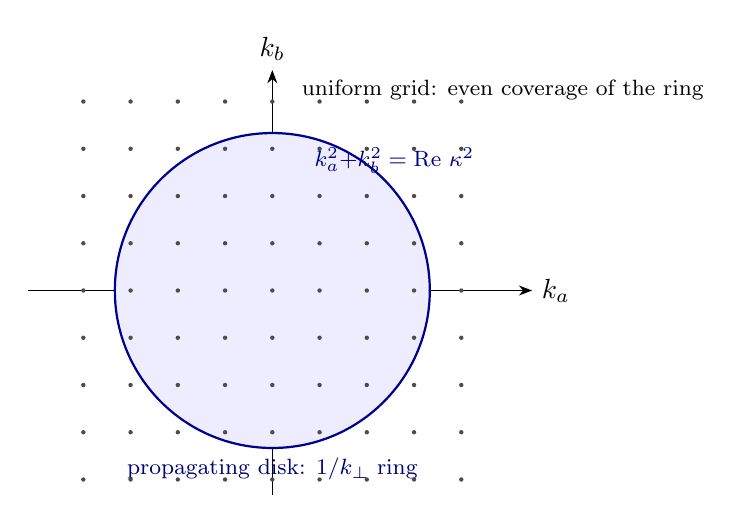
\begin{tikzpicture}[scale=1.0, >=Stealth]
  % axes
  \draw[->] (-3.1,0) -- (3.3,0) node[right] {$k_a$};
  \draw[->] (0,-2.6) -- (0,2.8) node[above] {$k_b$};
  % propagating disk
  \begin{scope}
    \clip (0,0) circle (2.0);
    \fill[blue!7] (-2.2,-2.2) rectangle (2.2,2.2);
  \end{scope}
  \draw[blue!55!black, thick] (0,0) circle (2.0);
  \node[blue!55!black] at (1.55,1.65) {\footnotesize $k_a^2{+}k_b^2=\Ree\,\kappa^2$};
  \node[blue!45!black] at (0.0,-2.0) [below] {\footnotesize propagating disk: $1/\kperp$ ring};
  % uniform grid of nodes
  \foreach \i in {-2.4,-1.8,...,2.4}{
    \foreach \j in {-2.4,-1.8,...,2.4}{
      \fill[black!70] (\i,\j) circle (0.028);
    }}
  \node[anchor=west, align=left] at (0.25,2.55) {\footnotesize uniform grid: even coverage of the ring};
\end{tikzpicture}
\caption{Quadrature of the angular-spectrum integral~\eqref{eq:weyl}. The
  kernel $1/\kperp$ is near-singular on the propagating circle
  $k_a^2+k_b^2=\Ree\,\kappa^2$ (the damping $\Imm\kappa>0$ keeps it finite). A
  dense \emph{uniform} grid (dots) covers the ring evenly and resolves it; a
  Gauss--Legendre rule of equal node count clusters toward the interval ends
  and under-resolves the ring, biasing the lattice sum.}
\label{fig:disk}
\end{figure}

%==============================================================================
\section{The lateral sweep: geometric resummation}
\label{sec:sweep}
%==============================================================================

Insert the swept-axis representation into the Bloch sum and isolate the
one-dimensional sublattice along the swept axis. With site index $i\in\mathbb Z$
at swept-axis position $\aL i$, swept-axis receiver coordinate $r_s$, and Bloch
phase $k_{\parallel,s}$, the swept-axis sum is
\begin{equation}
  S(\kperp,r_s)
  \;=\;\sum_{i\in\mathbb{Z}}
        e^{\,\ii\kperp\lvert r_s-\aL i\rvert}\,
        e^{\,\ii k_{\parallel,s}\,\aL i}.
  \label{eq:rowsum}
\end{equation}
The absolute value in the exponent is the only obstruction to this being a
plain geometric series, and it changes sign exactly once, at
$i_{0}=\lfloor r_s/\aL\rfloor$. Splitting the sum there removes the modulus:
\begin{equation}
  \begin{aligned}
    i\le i_{0}:&\quad r_s-\aL i\ge 0
      \ \Rightarrow\ e^{\,\ii\kperp r_s}\,p^{\,i},
      &p&=e^{\,\ii(k_{\parallel,s}-\kperp)\aL},\\[2pt]
    i> i_{0}:&\quad r_s-\aL i< 0
      \ \Rightarrow\ e^{-\ii\kperp r_s}\,q^{\,i},
      &q&=e^{\,\ii(k_{\parallel,s}+\kperp)\aL}.
  \end{aligned}
  \label{eq:pq}
\end{equation}
With the branch $\Imm\kperp>0$ of \S\ref{sec:residue} one has
$\lvert p\rvert=e^{\Imm(\kperp)\aL}>1$, so the left tail $i\to-\infty$
converges, and $\lvert q\rvert=e^{-\Imm(\kperp)\aL}<1$, so the right tail
$i\to+\infty$ converges. Each side is a geometric series, and~\eqref{eq:rowsum}
sums in closed form:
\begin{equation}
  \boxed{\;
  S(\kperp,r_s)
  \;=\;
  e^{\,\ii\kperp r_s}\,\frac{p^{\,i_{0}+1}}{p-1}
  \;+\;
  e^{-\ii\kperp r_s}\,\frac{q^{\,i_{0}+1}}{1-q}\;}
  \label{eq:rowclosed}
\end{equation}
This is the thesis cumulative-phase sweep (and the FFTProp row identity): the
phase of a propagating partial wave accumulates \emph{linearly} from site to
site, so the contribution of an entire row of the lattice is a single
closed-form expression rather than a truncated sum. The geometry of the split
is shown in Figure~\ref{fig:rowsplit}.

\begin{figure}[ht]
\centering
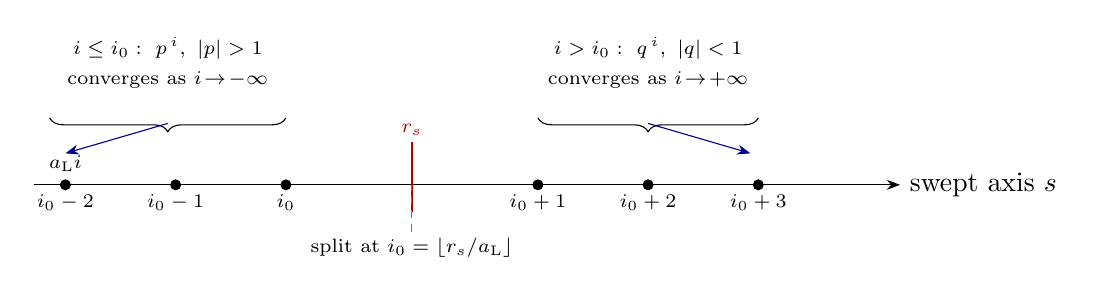
\begin{tikzpicture}[scale=1.0, >=Stealth]
  % swept axis
  \draw[->] (-5.4,0) -- (5.6,0) node[right] {swept axis $s$};
  % lattice sites
  \foreach \x/\lab in {-5/{i_0-2},-3.6/{i_0-1},-2.2/{i_0},1.0/{i_0+1},2.4/{i_0+2},3.8/{i_0+3}}{
    \fill (\x,0) circle (0.07);
    \node[below] at (\x,0) {\scriptsize $\lab$};
  }
  \node[above] at (-5,0.05) {\scriptsize $\aL i$};
  % receiver between i0 and i0+1
  \draw[red!70!black, thick] (-0.6,-0.35) -- (-0.6,0.55);
  \node[red!70!black, above] at (-0.6,0.5) {\scriptsize $r_s$};
  % left bracket: |p|>1, sum to -inf
  \draw[decorate, decoration={brace, amplitude=5pt}] (-2.2,0.85) -- (-5.2,0.85);
  \node[align=center] at (-3.7,1.55)
    {\scriptsize $i\le i_0:\ p^{\,i},\ \lvert p\rvert>1$\\[-1pt]
     \scriptsize converges as $i\!\to\!-\infty$};
  \draw[->, blue!55!black] (-3.7,0.78) -- (-5.0,0.4);
  % right bracket: |q|<1, sum to +inf
  \draw[decorate, decoration={brace, amplitude=5pt}] (3.8,0.85) -- (1.0,0.85);
  \node[align=center] at (2.4,1.55)
    {\scriptsize $i> i_0:\ q^{\,i},\ \lvert q\rvert<1$\\[-1pt]
     \scriptsize converges as $i\!\to\!+\infty$};
  \draw[->, blue!55!black] (2.4,0.78) -- (3.7,0.4);
  % split marker
  \draw[densely dashed, black!55] (-0.6,-0.6) -- (-0.6,0.0);
  \node[below] at (-0.6,-0.55) {\scriptsize split at $i_0=\lfloor r_s/\aL\rfloor$};
\end{tikzpicture}
\caption{The geometric row identity~\eqref{eq:rowclosed}. The modulus
  $\lvert r_s-\aL i\rvert$ in~\eqref{eq:rowsum} changes sign once, at
  $i_0=\lfloor r_s/\aL\rfloor$. To the left the ratio $p$ has
  $\lvert p\rvert>1$ and the sum to $-\infty$ converges; to the right
  $\lvert q\rvert<1$ and the sum to $+\infty$ converges. Each side is summed in
  closed form, so an entire lattice row is evaluated without truncation.}
\label{fig:rowsplit}
\end{figure}

%==============================================================================
\section{Poisson collapse and the depth quadrature}
\label{sec:poisson}
%==============================================================================

The orthogonal lateral direction (the ``reciprocal'' axis, with receiver
coordinate $r_r$ and Bloch phase $k_{\parallel,r}$) is still a sum over lattice
index $j$. Rather than sum it in real space, we apply Poisson summation to the
$j$-sum, which collapses the corresponding transverse integral in
\eqref{eq:weyl_z} onto the reciprocal lattice:
\begin{equation}
  \sum_{j\in\mathbb{Z}} e^{\,\ii k_a(r_r-\aL j)}\,e^{\,\ii k_{\parallel,r}\aL j}
  \;=\;\frac{2\pi}{\aL}\sum_{n\in\mathbb{Z}}
        \delta\!\left(k_a-k_{r,n}\right)\,e^{\,\ii k_{r,n} r_r},
  \qquad
  k_{r,n}=k_{\parallel,r}+\frac{2\pi n}{\aL}.
  \label{eq:poisson}
\end{equation}
The transverse $k_a$-integral is then done by the delta functions, fixing it to
the reciprocal-lattice values $k_{r,n}$. Combining the prefactor $\ii/8\pi^2$
of~\eqref{eq:weyl_z} with the factor $2\pi/\aL$ leaves $\ii/(4\pi\aL)$, and the
resummed intra-plane propagator is
\begin{equation}
  \boxed{\;
  G(\vr;\kappa)
  \;=\;\frac{\ii}{4\pi\,\aL}
       \sum_{n\in\mathbb{Z}} e^{\,\ii k_{r,n} r_r}
       \int \rd k_z\; e^{\,\ii k_z r_z}\,
       \frac{S\!\bigl(\kperp,r_s\bigr)}{\kperp}
       \;-\;g(\vr;\kappa),\;}
  \qquad
  \kperp=\sqrt{\kappa^{2}-k_{r,n}^{2}-k_z^{2}},
  \label{eq:fieldsweep}
\end{equation}
where $S$ is the closed-form row sum~\eqref{eq:rowclosed}, the final $g(\vr)$
subtracts the self ($i=j=0$) site that~\eqref{eq:blochsum} excludes, and the
swept/reciprocal assignment $(s,r)$ follows the dual-sweep rule~\eqref{eq:argmax}.

The three lattice directions are thus handled by three different and each
exact mechanisms: the swept lateral axis in closed form, the orthogonal lateral
axis by a fast reciprocal sum, and the depth by a one-dimensional quadrature.
The reciprocal sum over $n$ converges geometrically because for
$\lvert k_{r,n}\rvert>\lvert\kappa\rvert$ the wavenumber $\kperp$ is evanescent
and $S/\kperp$ decays like $e^{-\lvert k_{r,n}\rvert\,\lvert r_s\rvert}$; the
dual-sweep choice $\lvert r_s\rvert\ge\lvert r_r\rvert$ maximises this decay
rate. No spatial truncation is taken in either lateral direction. The structure
is summarised in Figure~\ref{fig:threeaxis}.

\begin{figure}[ht]
\centering
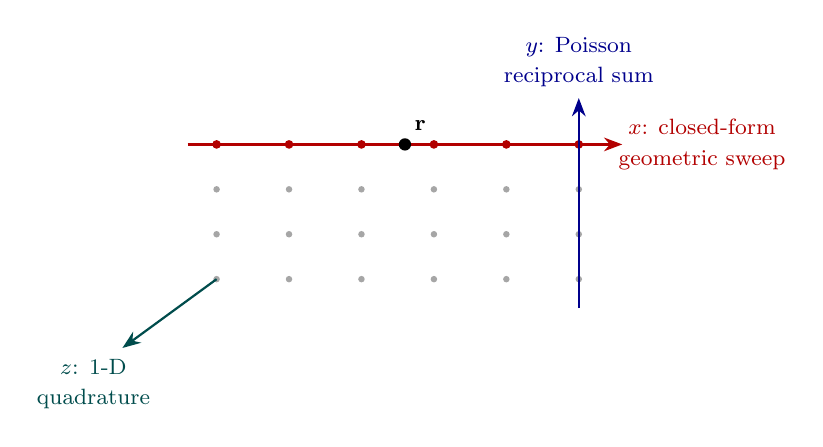
\begin{tikzpicture}[scale=0.92, >=Stealth]
  % planar lattice in x-y
  \foreach \i in {0,1,2,3,4,5}{
    \foreach \j in {0,1,2,3}{
      \fill[black!35] (\i*1.0, \j*0.62) circle (0.045);
    }}
  % swept-axis (x) row highlighted through receiver row
  \foreach \i in {0,1,2,3,4,5}{ \fill[red!70!black] (\i*1.0, 1.86) circle (0.06); }
  \draw[red!70!black, thick, ->] (-0.4,1.86) -- (5.6,1.86);
  \node[red!70!black, align=center] at (6.7,1.86)
    {\footnotesize $x$: closed-form\\[-1pt]\footnotesize geometric sweep};
  % reciprocal axis (y)
  \draw[blue!55!black, thick, ->] (5.0,-0.4) -- (5.0,2.5);
  \node[blue!55!black, align=center] at (5.0,3.0)
    {\footnotesize $y$: Poisson\\[-1pt]\footnotesize reciprocal sum};
  % depth axis (z) out of plane
  \draw[teal!60!black, thick, ->] (0,0) -- (-1.3,-0.95);
  \node[teal!60!black, align=center] at (-1.7,-1.45)
    {\footnotesize $z$: 1-D\\[-1pt]\footnotesize quadrature};
  % receiver
  \fill[black] (2.6,1.86) circle (0.085);
  \node[above right] at (2.6,1.92) {\footnotesize $\vr$};
\end{tikzpicture}
\caption{The spectral sweep over the planar lattice~\eqref{eq:fieldsweep}. The
  swept lateral axis (here $x$, red) is resummed in closed
  form~\eqref{eq:rowclosed}; the orthogonal lateral axis ($y$, blue) is a fast
  reciprocal sum after Poisson collapse~\eqref{eq:poisson}; the depth ($z$,
  out of plane) is a one-dimensional quadrature. The swept axis is chosen per
  receiver as $\arg\max(\lvert r_x\rvert,\lvert r_y\rvert)$.}
\label{fig:threeaxis}
\end{figure}

%==============================================================================
\section{From scalar to vector: the Kambe structure constants}
\label{sec:vector}
%==============================================================================

The elastic Bloch propagator $\vG_0^{\mathrm{vec}}(\kpar)$ is not an independent
object: an exact operator identity reduces it to the two scalar Helmholtz
lattice sums~\eqref{eq:blochsum} at the compressional and shear wavenumbers,
$\kappa_P$ and $\kappa_S$, dressed with standard angular (vector spherical
harmonic) coefficients. The irreducible content is therefore the set of scalar
\emph{lattice structure constants} $\Dqs$, the multipole coefficients of the
periodic field about a site. Establishing the spectral sweep at the scalar
level is hence sufficient: the vector propagator follows by contraction.

We extract $\Dqs$ by projecting the resummed field~\eqref{eq:fieldsweep} onto
spherical harmonics over a small sphere $\lvert\vr\rvert=\rho_0$ about a site,
\begin{equation}
  \Dqs^{\,\mathrm{sweep}}
  \;=\;\frac{1}{\ii\kappa\, j_q(\kappa\rho_0)}
        \oint G(\rho_0\hat{\mathbf{n}};\kappa)\,
        \overline{Y_q^{\,s}(\hat{\mathbf{n}})}\,\rd\Omega,
  \label{eq:project}
\end{equation}
which is to be compared with Kambe's addition-theorem evaluation of the same
constants as a direct real-space sum of outgoing spherical waves,
\begin{equation}
  \Dqs^{\,\mathrm{Kambe}}
  \;=\;\sum_{\vR\in\Lambda\setminus\{0\}}
        h_q^{(1)}\!\bigl(\kappa\lvert\vR\rvert\bigr)\,
        \overline{Y_q^{\,s}\!\bigl(\tfrac{\pi}{2},\phi_{\vR}\bigr)}\,
        e^{\,\ii\,\kpar\cdot\vR}.
  \label{eq:kambe}
\end{equation}
Both sums converge absolutely in the damped regime $\Imm\kappa>0$. The vector
projectors (regular/outgoing multipoles $\mathbf L,\mathbf M,\mathbf N$ in the
Cruzan/Stein normalisation, built from the radial and tangential vector
spherical harmonics) are ported and self-tested separately; once $\Dqs$ agrees,
the vector match is redundant. Figure~\ref{fig:repmap} places the spectral
sweep among the three representations of the same intra-plane propagator and
the Ewald route of companion~(I).

\begin{figure}[ht]
\centering
\resizebox{\textwidth}{!}{%
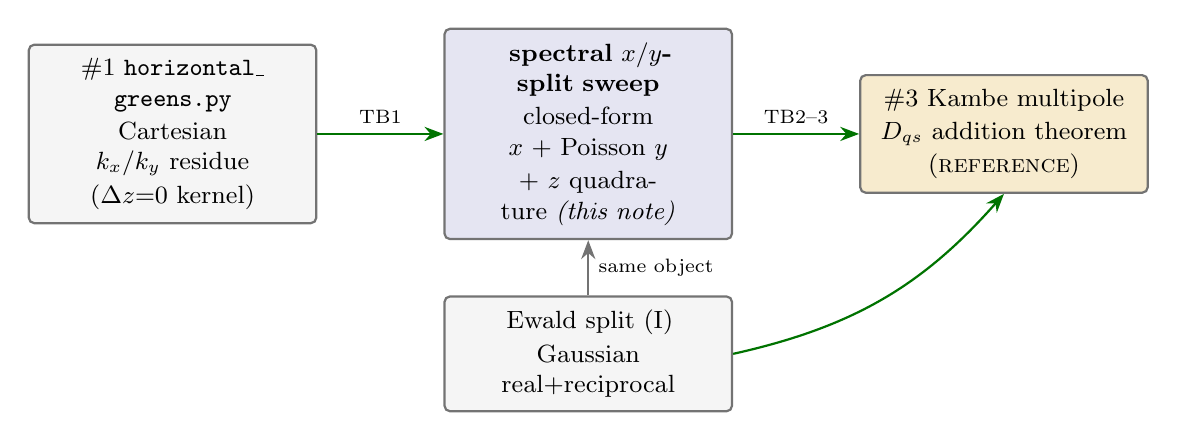
\begin{tikzpicture}[
  >=Stealth, node distance = 7mm and 16mm,
  rep/.style = {rectangle, rounded corners=2pt, draw=black!55, thick,
                align=center, text width=33mm, inner sep=5pt, font=\small},
  ref/.style = {rep, fill=Goldenrod!22},
  this/.style= {rep, fill=NavyBlue!10},
  alt/.style = {rep, fill=black!4},
  ok/.style  = {-{Stealth[length=2.4mm]}, thick, draw=green!45!black},
  pl/.style  = {-{Stealth[length=2.4mm]}, thick, draw=black!55}
]
  \node[alt] (hg)
    {\#1 \texttt{horizontal\_\allowbreak greens.py}\\[1pt]
     Cartesian $k_x/k_y$ residue\\[1pt]($\Delta z{=}0$ kernel)};
  \node[this, right=of hg] (sweep)
    {\textbf{spectral $x/y$-split sweep}\\[1pt]
     closed-form $x$ + Poisson $y$\\[1pt]+ $z$ quadrature \emph{(this note)}};
  \node[ref, right=of sweep] (kambe)
    {\#3 Kambe multipole\\[1pt]$\Dqs$ addition theorem\\[1pt](\textsc{reference})};
  \node[alt, below=of sweep] (ewald)
    {Ewald split (I)\\[1pt]Gaussian real$+$reciprocal};

  \draw[ok] (hg)   -- node[above,font=\scriptsize]{TB1} (sweep);
  \draw[ok] (sweep)-- node[above,font=\scriptsize]{TB2--3} (kambe);
  \draw[pl] (ewald)-- node[right,font=\scriptsize]{same object} (sweep);
  \draw[ok] (ewald.east) to[bend right=18]
            node[below,font=\scriptsize]{} (kambe.south);
\end{tikzpicture}%
}
\caption{The intra-plane propagator in three representations and two summation
  routes. The directional $x/y$-split sweep (centre, this note) is the
  spectral bridge: it extends the equal-depth Cartesian residue kernel of
  \texttt{horizontal\_\allowbreak greens.py} (\#1) to general depth and to the infinite
  lattice, and reproduces the Kambe multipole structure constants $\Dqs$ (\#3,
  the reference). The Ewald split of companion~(I) is an alternative summation
  of the same object. Green arrows are verified numerical equalities
  (\S\ref{sec:results}).}
\label{fig:repmap}
\end{figure}

%==============================================================================
\section{Numerical validation (damped regime)}
\label{sec:results}
%==============================================================================

The construction was validated as a chain of tracer-bullet checks in the damped
regime $\Imm\omega>0$, where both the real-space lattice sum and its spectral
resummation converge absolutely; the damping $\eta$ (with
$\omega=2\pi(1+\ii\eta)$) is a genuine physical attenuation, chosen per check
for fast convergence. Each check isolates one link in the chain
of Figure~\ref{fig:repmap}. Backgound $\alpha=5,\ \beta=3$; lattice
pitch $\aL=2$; Bloch vector $\kpar=(0.2,0.1)$.

\begin{table}[ht]
\centering
\caption{Damped-regime validation of the intra-plane spectral sweep. Each row
  reports the relative agreement of one link in the chain
  \texttt{horizontal\_greens} $\to$ residue $\to$ sweep $\to$ Kambe.}
\label{tab:results}
\small
\begin{tabularx}{\textwidth}{@{}l X X l@{}}
\toprule
Check & What is compared & Statement & Residual\\
\midrule
TB1  & residue kernel vs.\ exact, in-plane
     & $G^{\mathrm{res}}_{ik}(\vR)=G^{\mathrm{exact}}_{ik}(\vR)$ at lattice vectors
     & $2.9\times10^{-5}$\\
TB2a & general-$z$ residue vs.\ exact
     & \eqref{eq:weyl_z} off-plane
     & $1.3\times10^{-4}$\\
TB2b & structure constants, residue vs.\ Kambe
     & $\Dqs^{\mathrm{sweep}}=\Dqs^{\mathrm{Kambe}}$, $\kappa_P/\kappa_S$
     & $2.3\times10^{-4}\,/\,2.5\times10^{-7}$\\
TB3a & row resummation vs.\ brute
     & \eqref{eq:rowclosed} $=$ truncated~\eqref{eq:rowsum}, $M{=}4000$
     & $2\times10^{-15}$\\
TB2c & vector $\mathbf L/\mathbf M/\mathbf N$ projector
     & self-consistency (reconstruct own coefficients)
     & $6\times10^{-16}$\\
\bottomrule
\end{tabularx}
\end{table}

The two extremes of Table~\ref{tab:results} carry the most information. The row
identity TB3a is exact to machine precision ($2\times10^{-15}$): the closed
form~\eqref{eq:rowclosed} \emph{is} the brute lattice sum, with no approximation
beyond floating point. At the other end, TB2b confirms the substantive
cross-code statement, that the spectral-sweep structure constants equal the
Kambe addition-theorem constants; the residual there is set by the angular
quadrature on the projection sphere and by the residue quadrature of the
propagating disk (Figure~\ref{fig:disk}), and tightens with node count. An
intermediate gate (not shown) confirms that projecting the \emph{exact} lattice
field with the same projector returns the Kambe constants to $10^{-13}$, so the
small TB2b residual is quadrature, not a representation error. The
$\kappa_S$ residual is far smaller than $\kappa_P$ because the larger shear
wavenumber places the propagating disk where the fixed uniform grid resolves it
more finely.

The full sweep-resummed field of \eqref{eq:fieldsweep} (TB3b) reproduces both
the brute lattice sum and the Kambe constants within tolerance, confirming that
the closed-form row, the Poisson reciprocal sum, and the depth quadrature
compose into the infinite-lattice limit that Kambe converges to.

%==============================================================================
\section{Relationship to the companion constructions}
\label{sec:lineage}
%==============================================================================

The spectral sweep and the Ewald split of companion~(I) compute the same
conditionally convergent object~\eqref{eq:blochsum} by different analytic
continuations. Ewald splits each term into a Gaussian-damped real-space part and
a Gaussian-damped reciprocal-space part, both absolutely convergent for any
geometry; it is the method of choice for a fully irregular evaluation and is
agnostic to direction. The spectral sweep instead exploits the one-dimensional
periodicity of a lattice \emph{row}: along the swept axis the sum is not merely
accelerated but eliminated, replaced by the closed form~\eqref{eq:rowclosed},
and only the orthogonal lateral direction carries a (reciprocal) sum. This is
exactly the structure that makes it a matrix--vector product in companion~(III):
the directional partial-wave sweep there is the operator version
of~\eqref{eq:fieldsweep}, applied across the voxel grid, with the depth handled
by the Kennett recursion between planes rather than by quadrature.

In the language of the three representations (Figure~\ref{fig:repmap}), the
sweep is the bridge that promotes the equal-depth Cartesian residue kernel of
\texttt{horizontal\_\allowbreak greens.py} to the general-depth infinite-lattice propagator,
and validates it against the Kambe multipole reference without ever forming a
truncated real-space lattice sum.

\end{document}
